\documentclass[a4paper,12pt]{article}
\usepackage[T2A]{fontenc}
\usepackage[utf8]{inputenc}
\usepackage[russian]{babel}
\usepackage{amsmath,amssymb}
\usepackage[margin=2cm]{geometry}
\usepackage{multirow}
\usepackage{graphicx}
\usepackage{float}
\usepackage{fvextra}
\usepackage[hidelinks]{hyperref}

% BEGIN GENERATED RESULTS
\newcommand{\ErlangOrder}{2}
\newcommand{\ErlangRate}{0{,}011362}
\newcommand{\UnroundedOrder}{2{,}051}
\newcommand{\OriginalMean}{176{,}03}
\newcommand{\OriginalVariance}{15108{,}4}
\newcommand{\OriginalCV}{0{,}698}
\newcommand{\TheoreticalVariance}{15493{,}7}
\newcommand{\CdfDistance}{0{,}049}
\newcommand{\CrossCorrelation}{-0{,}0372}
\newcommand{\OriginalMaxACF}{0{,}0656}
\newcommand{\GeneratedMaxACF}{0{,}0683}
\newcommand{\MeanDeviation}{8{,}7\,\%}
\newcommand{\VarianceDeviation}{14{,}5\,\%}
\newcommand{\StdDeviation}{7{,}0\,\%}
\newcommand{\CVDeviation}{1{,}6\,\%}
\newcommand{\FirstMeanInterval}{47{,}00}
\newcommand{\LastMeanInterval}{13{,}91}
\newcommand{\GeneratorSeed}{132}
\newcommand{\OriginalRows}{%
\multirow{2}{*}{\textbf{Мат.ож.}} & Знач. & 154{,}67 & 149{,}80 & 161{,}55 & 182{,}02 & 178{,}69 & \multirow{2}{*}{176{,}03} \\ \cline{2-7}
 & \% & 12{,}1\,\% & 14{,}9\,\% & 8{,}2\,\% & 3{,}4\,\% & 1{,}5\,\% &  \\ \hline
\multirow{2}{*}{Дов. инт. (0,9)} & Знач. & $\pm 39{,}40$ & $\pm 29{,}72$ & $\pm 23{,}68$ & $\pm 19{,}97$ & $\pm 14{,}45$ & \multirow{2}{*}{$\pm 11{,}66$} \\ \cline{2-7}
 & \% & 237{,}9\,\% & 154{,}9\,\% & 103{,}1\,\% & 71{,}3\,\% & 23{,}9\,\% &  \\ \hline
\multirow{2}{*}{Дов. инт. (0,95)} & Знач. & $\pm 47{,}00$ & $\pm 35{,}46$ & $\pm 28{,}25$ & $\pm 23{,}82$ & $\pm 17{,}24$ & \multirow{2}{*}{$\pm 13{,}91$} \\ \cline{2-7}
 & \% & 237{,}9\,\% & 154{,}9\,\% & 103{,}1\,\% & 71{,}3\,\% & 23{,}9\,\% &  \\ \hline
\multirow{2}{*}{Дов. инт. (0,99)} & Знач. & $\pm 61{,}77$ & $\pm 46{,}60$ & $\pm 37{,}13$ & $\pm 31{,}31$ & $\pm 22{,}66$ & \multirow{2}{*}{$\pm 18{,}28$} \\ \cline{2-7}
 & \% & 237{,}9\,\% & 154{,}9\,\% & 103{,}1\,\% & 71{,}3\,\% & 23{,}9\,\% &  \\ \hline
\multirow{2}{*}{\textbf{Дисперсия}} & Знач. & 5749{,}6 & 6545{,}2 & 10386{,}0 & 14771{,}9 & 15471{,}7 & \multirow{2}{*}{15108{,}4} \\ \cline{2-7}
 & \% & 61{,}9\,\% & 56{,}7\,\% & 31{,}3\,\% & 2{,}2\,\% & 2{,}4\,\% &  \\ \hline
\multirow{2}{*}{\textbf{С.к.о.}} & Знач. & 75{,}83 & 80{,}90 & 101{,}91 & 121{,}54 & 124{,}39 & \multirow{2}{*}{122{,}92} \\ \cline{2-7}
 & \% & 38{,}3\,\% & 34{,}2\,\% & 17{,}1\,\% & 1{,}1\,\% & 1{,}2\,\% &  \\ \hline
\multirow{2}{*}{\textbf{К-т вариации}} & Знач. & 0{,}490 & 0{,}540 & 0{,}631 & 0{,}668 & 0{,}696 & \multirow{2}{*}{0{,}698} \\ \cline{2-7}
 & \% & 29{,}8\,\% & 22{,}7\,\% & 9{,}7\,\% & 4{,}4\,\% & 0{,}3\,\% &  \\ \hline
}
\newcommand{\GeneratedRows}{%
\multirow{2}{*}{\textbf{Мат.ож.}} & Знач. & 230{,}12 & 197{,}59 & 200{,}97 & 195{,}79 & 198{,}76 & 191{,}41 \\ \cline{2-8}
 & \% & 48{,}8\,\% & 31{,}9\,\% & 24{,}4\,\% & 7{,}6\,\% & 11{,}2\,\% & 8{,}7\,\% \\ \hline
\multirow{2}{*}{Дов. инт. (0,9)} & Знач. & $\pm 88{,}63$ & $\pm 53{,}11$ & $\pm 29{,}71$ & $\pm 21{,}61$ & $\pm 16{,}20$ & $\pm 12{,}48$ \\ \cline{2-8}
 & \% & 125{,}0\,\% & 78{,}7\,\% & 25{,}4\,\% & 8{,}2\,\% & 12{,}1\,\% & 7{,}0\,\% \\ \hline
\multirow{2}{*}{Дов. инт. (0,95)} & Знач. & $\pm 105{,}73$ & $\pm 63{,}36$ & $\pm 35{,}44$ & $\pm 25{,}79$ & $\pm 19{,}32$ & $\pm 14{,}88$ \\ \cline{2-8}
 & \% & 125{,}0\,\% & 78{,}7\,\% & 25{,}4\,\% & 8{,}2\,\% & 12{,}1\,\% & 7{,}0\,\% \\ \hline
\multirow{2}{*}{Дов. инт. (0,99)} & Знач. & $\pm 138{,}96$ & $\pm 83{,}27$ & $\pm 46{,}57$ & $\pm 33{,}89$ & $\pm 25{,}39$ & $\pm 19{,}56$ \\ \cline{2-8}
 & \% & 125{,}0\,\% & 78{,}7\,\% & 25{,}4\,\% & 8{,}2\,\% & 12{,}1\,\% & 7{,}0\,\% \\ \hline
\multirow{2}{*}{\textbf{Дисперсия}} & Знач. & 29098{,}6 & 20897{,}4 & 16344{,}4 & 17307{,}2 & 19433{,}3 & 17299{,}9 \\ \cline{2-8}
 & \% & 406{,}1\,\% & 219{,}3\,\% & 57{,}4\,\% & 17{,}2\,\% & 25{,}6\,\% & 14{,}5\,\% \\ \hline
\multirow{2}{*}{\textbf{С.к.о.}} & Знач. & 170{,}58 & 144{,}56 & 127{,}85 & 131{,}56 & 139{,}40 & 131{,}53 \\ \cline{2-8}
 & \% & 125{,}0\,\% & 78{,}7\,\% & 25{,}4\,\% & 8{,}2\,\% & 12{,}1\,\% & 7{,}0\,\% \\ \hline
\multirow{2}{*}{\textbf{К-т вариации}} & Знач. & 0{,}741 & 0{,}732 & 0{,}636 & 0{,}672 & 0{,}701 & 0{,}687 \\ \cline{2-8}
 & \% & 51{,}2\,\% & 35{,}5\,\% & 0{,}8\,\% & 0{,}6\,\% & 0{,}8\,\% & 1{,}6\,\% \\ \hline
}
\newcommand{\AutocorrelationRows}{%
\textbf{К-т АК} для задан. \textbf{ЧП} & -0{,}0267 & -0{,}0076 & 0{,}0656 & 0{,}0585 & -0{,}0434 & -0{,}0141 & 0{,}0387 & -0{,}0561 & -0{,}0619 & 0{,}0251 \\ \hline
\textbf{К-т АК} для сгенерир. \textbf{ЧП} & 0{,}0600 & -0{,}0350 & -0{,}0024 & -0{,}0633 & 0{,}0165 & -0{,}0430 & -0{,}0683 & 0{,}0088 & 0{,}0523 & -0{,}0202 \\ \hline
\textit{\%} & 324{,}5\,\% & 362{,}6\,\% & 103{,}6\,\% & 208{,}1\,\% & 138{,}0\,\% & 204{,}7\,\% & 276{,}4\,\% & 115{,}7\,\% & 184{,}5\,\% & 180{,}3\,\% \\ \hline
}
% END GENERATED RESULTS
\newcommand{\SampleHeader}{\textbf{Характеристика} & &
  \multicolumn{6}{c|}{\textbf{Количество случайных величин}} \\ \cline{2-8}
  & & \textbf{10} & \textbf{20} & \textbf{50} & \textbf{100} &
  \textbf{200} & \textbf{300} \\ \hline}

\begin{document}
\hypersetup{pageanchor=false}
\begin{titlepage}
  \centering
  Федеральное государственное автономное образовательное учреждение высшего
  образования «Национальный исследовательский университет ИТМО»\par
  \vspace{1cm}
  Факультет программной инженерии и компьютерной техники\par
  \vfill
  {\large Дисциплина «Моделирование»\par}
  \vspace{0.5cm}
  Лабораторная работа №~1\par
  «Обработка результатов измерений: статистический анализ числовой последовательности»\par
  Вариант 132\par
  \vfill
  \begin{flushright}
    \textbf{Выполнил}\par
    Козаченко Данил Александрович\par
    Группа P3312\par
    \medskip
    \textbf{Проверил}\par
    Тропченко Андрей Александрович
  \end{flushright}
  \vspace{2cm}
  Санкт-Петербург\par
  2026~г.
\end{titlepage}

\hypersetup{pageanchor=true}
\tableofcontents
\clearpage

\section{Цель работы}
Изучить методы статистического анализа результатов измерений, оценить числовые
характеристики заданной последовательности, исследовать её автокорреляцию и
аппроксимировать закон распределения по двум начальным моментам. Сгенерировать
последовательность по выбранному закону и сравнить её с заданной.

\section{Анализ заданной числовой последовательности}

\subsection{Оценки числовых характеристик}
Для каждого объёма $n$ использованы первые $n$ наблюдений. Выборочное среднее
$\bar{x}$, несмещённая оценка дисперсии $s^2$ и коэффициент вариации $V$ рассчитаны
по формулам
\[
  \bar{x}=\frac{1}{n}\sum_{i=1}^{n}x_i,\qquad
  s^2=\frac{1}{n-1}\sum_{i=1}^{n}(x_i-\bar{x})^2,\qquad
  V=\frac{s}{\bar{x}},\quad s=\sqrt{s^2}.
\]
Приближённый доверительный интервал для математического ожидания имеет вид
$\bar{x}\pm\varepsilon_p$, где $\varepsilon_p=t_p s/\sqrt{n}$. По таблице 1
методических материалов для $p=0{,}90$, $0{,}95$ и $0{,}99$ взяты
$t_p=1{,}643$, $1{,}960$ и $2{,}576$ соответственно. При малых $n$ точность
нормального приближения ограничена.

\begin{table}[H]
  \centering
  \hfill Форма 1\par
  Характеристики \textbf{\textit{заданной}} ЧП (\textbf{вариант 132})\par\smallskip
  \resizebox{\textwidth}{!}{%
    \begin{tabular}{|c|c|*{6}{c|}}
      \hline
      \SampleHeader
      \OriginalRows
    \end{tabular}%
  }\par\smallskip
  {\small \%~--- относительные отклонения рассчитанных значений от значений,
  полученных для выборки из трёхсот величин.\par}
\end{table}

Для каждой характеристики $a$ в форме 1 приведено отклонение
$100\,|a_n-a_{300}|/|a_{300}|$ в процентах. При увеличении объёма выборки
от 10 до 300 доверительный полуинтервал при $p=0{,}95$ уменьшился
с $\FirstMeanInterval$ до $\LastMeanInterval$. При $n=200$ оценки среднего,
дисперсии и СКО отличаются от оценок для $n=300$ менее чем на $3\,\%$.

\clearpage
\subsection{График значений и характер последовательности}
\begin{figure}[H]
  \centering
  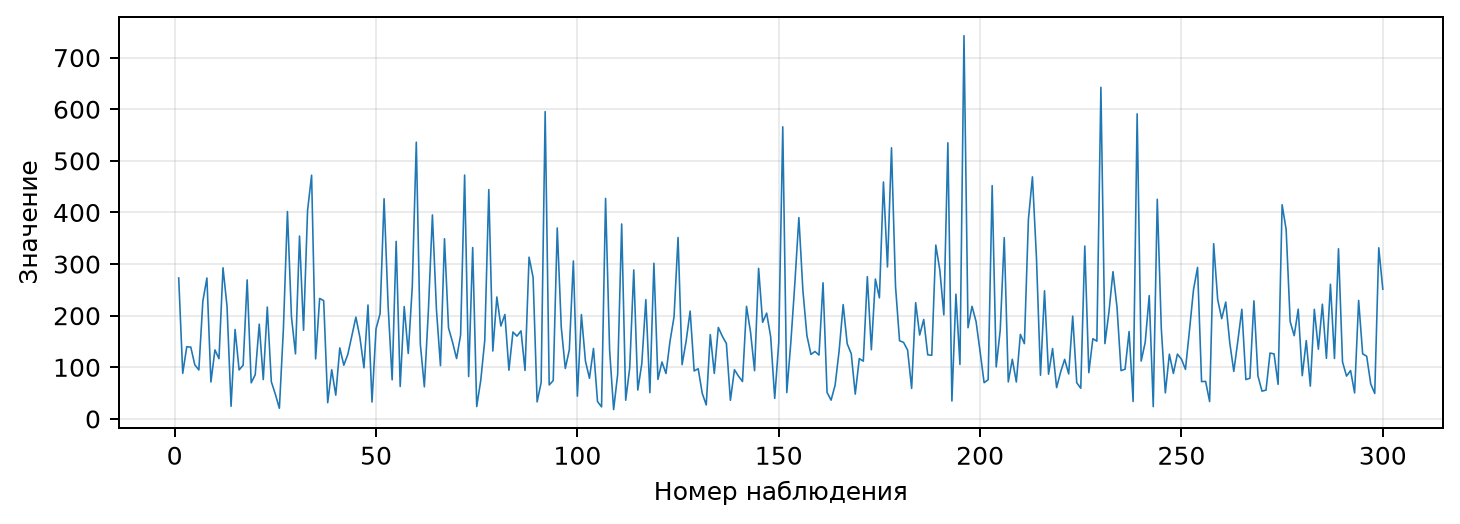
\includegraphics[width=0.78\textwidth]{graph1.png}
  \caption{График 1. Значения заданной числовой последовательности}
  \label{fig:original}
\end{figure}

На графике последовательность немонотонна. Визуально выраженный тренд
и повторяющийся период не обнаружены.

\subsection{Автокорреляционный анализ}
Для каждой последовательности $z_1,\dots,z_N$ при $N=300$ вычислены коэффициенты
автокорреляции со сдвигом $h$ от 1 до 10:
\[
  r_h = \frac{\sum_{i=1}^{N-h}(z_i-\bar z)(z_{i+h}-\bar z)}
                {\sum_{i=1}^{N}(z_i-\bar z)^2}.
\]

\begin{table}[H]
  \centering
  \hfill Форма 3\par
  Коэффициенты автокорреляции\par\smallskip
  \resizebox{\textwidth}{!}{%
    \begin{tabular}{|c|*{10}{c|}}
      \hline
      \textbf{Сдвиг ЧП} & 1 & 2 & 3 & 4 & 5 & 6 & 7 & 8 & 9 & 10 \\ \hline
      \AutocorrelationRows
    \end{tabular}%
  }
\end{table}

\begin{figure}[H]
  \centering
  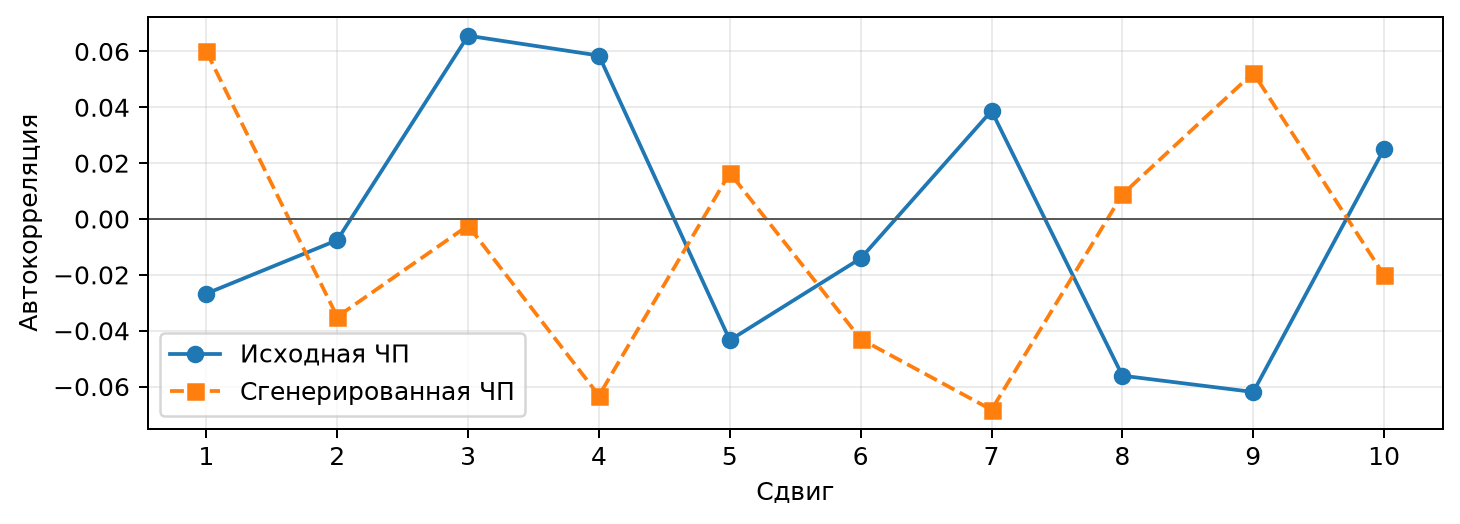
\includegraphics[width=0.78\textwidth]{autocorr.png}
  \caption{Коррелограмма заданной и сгенерированной последовательностей}
  \label{fig:acf}
\end{figure}

Максимальные значения $|r_h|$ на проверенных сдвигах составляют
$\OriginalMaxACF$ для заданной ЧП и $\GeneratedMaxACF$ для сгенерированной.
На этих сдвигах заметной линейной связи не обнаружено. Такой результат
согласуется со случайным характером заданной последовательности.
В форме 3 проценты рассчитаны относительно модулей исходных
коэффициентов. При исходных коэффициентах, близких к нулю, даже малые
разности дают большие относительные отклонения.

\clearpage
\section{Аппроксимация закона распределения}

\subsection{Гистограмма распределения частот}
\begin{figure}[H]
  \centering
  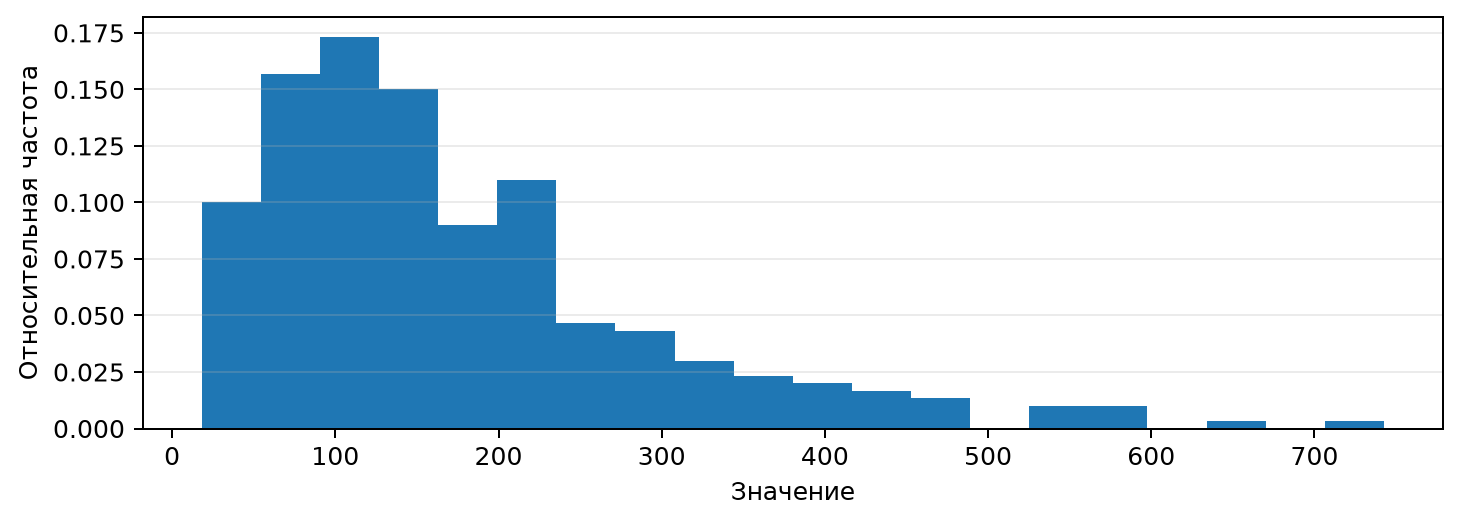
\includegraphics[width=0.9\textwidth]{graph2.png}
  \caption{График 2. Гистограмма относительных частот заданной ЧП}
  \label{fig:frequency}
\end{figure}

Большинство наблюдений сосредоточено в левой части гистограммы.
Более редкие большие значения образуют правый хвост.

\subsection{Выбор и оценка аппроксимирующего закона}
Для заданной ЧП $\bar{x}=\OriginalMean$, $s^2=\OriginalVariance$ и
$V\approx\OriginalCV$. Значение $V$ близко к $1/\sqrt{2}$, поэтому выбрано
распределение Эрланга второго порядка.

Параметры оценены по среднему и дисперсии. Эти оценки соответствуют первым двум
начальным моментам через соотношение $\mathrm{E}[X^2]=\mathrm{Var}(X)+(\mathrm{E}[X])^2$.
Для распределения Эрланга с порядком $k$ и интенсивностью $\lambda$ среднее
равно $k/\lambda$, а дисперсия~--- $k/\lambda^2$. Отсюда
\[
  k=\operatorname{round}\!\left(\frac{\bar{x}^2}{s^2}\right)
    =\operatorname{round}(\UnroundedOrder)=\ErlangOrder,\qquad
  \lambda=\frac{k}{\bar{x}}\approx\ErlangRate.
\]
При целочисленном $k$ среднее аппроксимирующего закона совпадает с выборочным,
а теоретическая дисперсия $\TheoreticalVariance$ близка к оценке
$\OriginalVariance$.

\begin{figure}[H]
  \centering
  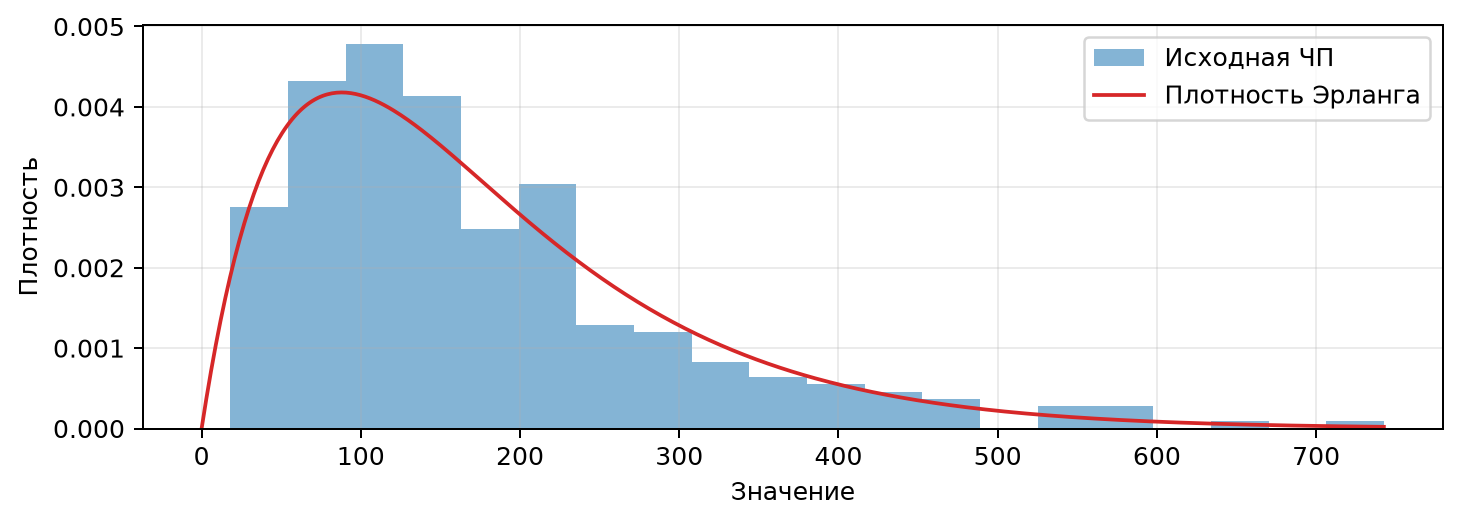
\includegraphics[width=0.9\textwidth]{graph3.png}
  \caption{График 3. Гистограмма заданной ЧП и плотность распределения Эрланга}
  \label{fig:density}
\end{figure}

Гистограмма на графике 3 нормирована до единичной площади. Теоретическая кривая
воспроизводит правую асимметрию. Максимальное абсолютное различие между
эмпирической и теоретической функциями распределения составляет
$\CdfDistance$.

\clearpage
\section{Генерация и сравнение последовательностей}
Каждое из 300 значений сгенерировано как сумма $k$ независимых величин
с экспоненциальным распределением интенсивности $\lambda$. В программе
использовано фиксированное начальное значение генератора $\GeneratorSeed$,
чтобы воспроизводить одну и ту же выборку при запуске.

\begin{table}[H]
  \centering
  \hfill Форма 2\par
  Характеристики \textbf{\textit{сгенерированной}} случайной ЧП\par\smallskip
  \resizebox{\textwidth}{!}{%
    \begin{tabular}{|c|c|*{6}{c|}}
      \hline
      \multicolumn{8}{|l|}{\textbf{\textit{Закон распределения:}}
        нормированный закон Эрланга, $k=\ErlangOrder$, $\lambda\approx\ErlangRate$} \\ \hline
      \SampleHeader
      \GeneratedRows
    \end{tabular}%
  }\par\smallskip
  {\small \%~--- относительные отклонения характеристик сгенерированной случайной
  последовательности от одноимённых значений заданной числовой последовательности.\par}
\end{table}

Проценты в форме 2 показывают абсолютные относительные отклонения от
одноимённых характеристик заданной ЧП при том же $n$. При $n=300$
среднее, дисперсия, СКО и коэффициент вариации отличаются соответственно
на \MeanDeviation, \VarianceDeviation, \StdDeviation{} и \CVDeviation.

\clearpage
\subsection{Сравнение значений и распределений}
\begin{figure}[H]
  \centering
  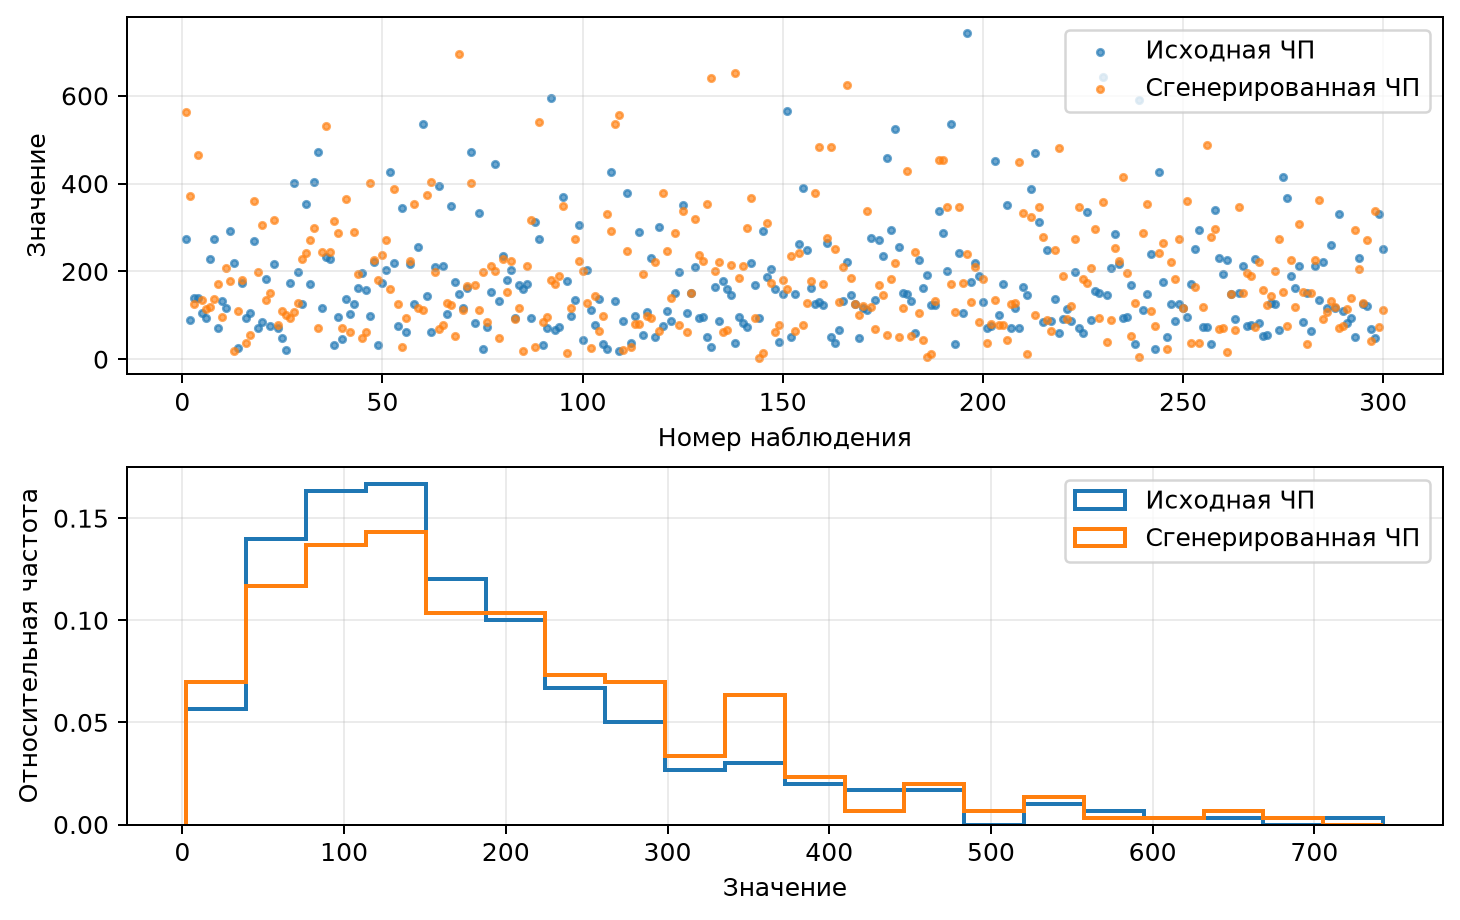
\includegraphics[width=0.9\textwidth]{comparison.png}
  \caption{Значения и гистограммы заданной и сгенерированной последовательностей}
  \label{fig:comparison}
\end{figure}

Гистограммы построены по общим интервалам. Оба ряда имеют правый хвост,
но на отдельных интервалах относительные частоты различаются. График значений
показывает разброс обеих последовательностей по номерам наблюдений.

\subsection{Взаимная корреляция}
Для пар наблюдений с одинаковым номером коэффициент корреляции Пирсона равен
\[
 r_{xy} =
 \frac{\sum_{i=1}^{N}(x_i-\bar x)(y_i-\bar y)}
 {\sqrt{\sum_{i=1}^{N}(x_i-\bar x)^2\sum_{i=1}^{N}(y_i-\bar y)^2}}
 \approx \CrossCorrelation.
\]
В рассмотренной паре последовательностей заметной линейной связи между
наблюдениями с одинаковыми номерами не обнаружено.

\section{Вывод}
График и малые значения автокорреляции на сдвигах 1--10 согласуются
со случайным характером заданной последовательности. При увеличении объёма
выборки доверительные интервалы для среднего сужаются. Распределение Эрланга
второго порядка описывает общую форму исходного распределения и близко
к нему по дисперсии. При $n=300$ наибольшее относительное различие между
характеристиками двух выборок получено для дисперсии. Корреляция между рядами
близка к нулю.

\clearpage
\appendix
\section{Листинг программы}
Программа считывает исходные данные, рассчитывает характеристики обеих
последовательностей и сохраняет таблицы и графики для сборки отчёта.
Для запуска нужны Python, NumPy, SciPy и Matplotlib.
\VerbatimInput[fontsize=\footnotesize,numbers=left,breaklines]{../main.py}

\end{document}
